\documentclass[]{article}
\usepackage{lmodern}
\usepackage{amssymb,amsmath}
\usepackage{ifxetex,ifluatex}
\usepackage{fixltx2e} % provides \textsubscript
\ifnum 0\ifxetex 1\fi\ifluatex 1\fi=0 % if pdftex
  \usepackage[T1]{fontenc}
  \usepackage[utf8]{inputenc}
\else % if luatex or xelatex
  \ifxetex
    \usepackage{mathspec}
  \else
    \usepackage{fontspec}
  \fi
  \defaultfontfeatures{Ligatures=TeX,Scale=MatchLowercase}
\fi
% use upquote if available, for straight quotes in verbatim environments
\IfFileExists{upquote.sty}{\usepackage{upquote}}{}
% use microtype if available
\IfFileExists{microtype.sty}{%
\usepackage{microtype}
\UseMicrotypeSet[protrusion]{basicmath} % disable protrusion for tt fonts
}{}
\usepackage[margin=1in]{geometry}
\usepackage{hyperref}
\hypersetup{unicode=true,
            pdftitle={Chicago Crime Data Analysis},
            pdfauthor={201081646},
            pdfborder={0 0 0},
            breaklinks=true}
\urlstyle{same}  % don't use monospace font for urls
\usepackage{color}
\usepackage{fancyvrb}
\newcommand{\VerbBar}{|}
\newcommand{\VERB}{\Verb[commandchars=\\\{\}]}
\DefineVerbatimEnvironment{Highlighting}{Verbatim}{commandchars=\\\{\}}
% Add ',fontsize=\small' for more characters per line
\usepackage{framed}
\definecolor{shadecolor}{RGB}{248,248,248}
\newenvironment{Shaded}{\begin{snugshade}}{\end{snugshade}}
\newcommand{\KeywordTok}[1]{\textcolor[rgb]{0.13,0.29,0.53}{\textbf{{#1}}}}
\newcommand{\DataTypeTok}[1]{\textcolor[rgb]{0.13,0.29,0.53}{{#1}}}
\newcommand{\DecValTok}[1]{\textcolor[rgb]{0.00,0.00,0.81}{{#1}}}
\newcommand{\BaseNTok}[1]{\textcolor[rgb]{0.00,0.00,0.81}{{#1}}}
\newcommand{\FloatTok}[1]{\textcolor[rgb]{0.00,0.00,0.81}{{#1}}}
\newcommand{\ConstantTok}[1]{\textcolor[rgb]{0.00,0.00,0.00}{{#1}}}
\newcommand{\CharTok}[1]{\textcolor[rgb]{0.31,0.60,0.02}{{#1}}}
\newcommand{\SpecialCharTok}[1]{\textcolor[rgb]{0.00,0.00,0.00}{{#1}}}
\newcommand{\StringTok}[1]{\textcolor[rgb]{0.31,0.60,0.02}{{#1}}}
\newcommand{\VerbatimStringTok}[1]{\textcolor[rgb]{0.31,0.60,0.02}{{#1}}}
\newcommand{\SpecialStringTok}[1]{\textcolor[rgb]{0.31,0.60,0.02}{{#1}}}
\newcommand{\ImportTok}[1]{{#1}}
\newcommand{\CommentTok}[1]{\textcolor[rgb]{0.56,0.35,0.01}{\textit{{#1}}}}
\newcommand{\DocumentationTok}[1]{\textcolor[rgb]{0.56,0.35,0.01}{\textbf{\textit{{#1}}}}}
\newcommand{\AnnotationTok}[1]{\textcolor[rgb]{0.56,0.35,0.01}{\textbf{\textit{{#1}}}}}
\newcommand{\CommentVarTok}[1]{\textcolor[rgb]{0.56,0.35,0.01}{\textbf{\textit{{#1}}}}}
\newcommand{\OtherTok}[1]{\textcolor[rgb]{0.56,0.35,0.01}{{#1}}}
\newcommand{\FunctionTok}[1]{\textcolor[rgb]{0.00,0.00,0.00}{{#1}}}
\newcommand{\VariableTok}[1]{\textcolor[rgb]{0.00,0.00,0.00}{{#1}}}
\newcommand{\ControlFlowTok}[1]{\textcolor[rgb]{0.13,0.29,0.53}{\textbf{{#1}}}}
\newcommand{\OperatorTok}[1]{\textcolor[rgb]{0.81,0.36,0.00}{\textbf{{#1}}}}
\newcommand{\BuiltInTok}[1]{{#1}}
\newcommand{\ExtensionTok}[1]{{#1}}
\newcommand{\PreprocessorTok}[1]{\textcolor[rgb]{0.56,0.35,0.01}{\textit{{#1}}}}
\newcommand{\AttributeTok}[1]{\textcolor[rgb]{0.77,0.63,0.00}{{#1}}}
\newcommand{\RegionMarkerTok}[1]{{#1}}
\newcommand{\InformationTok}[1]{\textcolor[rgb]{0.56,0.35,0.01}{\textbf{\textit{{#1}}}}}
\newcommand{\WarningTok}[1]{\textcolor[rgb]{0.56,0.35,0.01}{\textbf{\textit{{#1}}}}}
\newcommand{\AlertTok}[1]{\textcolor[rgb]{0.94,0.16,0.16}{{#1}}}
\newcommand{\ErrorTok}[1]{\textcolor[rgb]{0.64,0.00,0.00}{\textbf{{#1}}}}
\newcommand{\NormalTok}[1]{{#1}}
\usepackage{graphicx,grffile}
\makeatletter
\def\maxwidth{\ifdim\Gin@nat@width>\linewidth\linewidth\else\Gin@nat@width\fi}
\def\maxheight{\ifdim\Gin@nat@height>\textheight\textheight\else\Gin@nat@height\fi}
\makeatother
% Scale images if necessary, so that they will not overflow the page
% margins by default, and it is still possible to overwrite the defaults
% using explicit options in \includegraphics[width, height, ...]{}
\setkeys{Gin}{width=\maxwidth,height=\maxheight,keepaspectratio}
\IfFileExists{parskip.sty}{%
\usepackage{parskip}
}{% else
\setlength{\parindent}{0pt}
\setlength{\parskip}{6pt plus 2pt minus 1pt}
}
\setlength{\emergencystretch}{3em}  % prevent overfull lines
\providecommand{\tightlist}{%
  \setlength{\itemsep}{0pt}\setlength{\parskip}{0pt}}
\setcounter{secnumdepth}{5}
% Redefines (sub)paragraphs to behave more like sections
\ifx\paragraph\undefined\else
\let\oldparagraph\paragraph
\renewcommand{\paragraph}[1]{\oldparagraph{#1}\mbox{}}
\fi
\ifx\subparagraph\undefined\else
\let\oldsubparagraph\subparagraph
\renewcommand{\subparagraph}[1]{\oldsubparagraph{#1}\mbox{}}
\fi

%%% Use protect on footnotes to avoid problems with footnotes in titles
\let\rmarkdownfootnote\footnote%
\def\footnote{\protect\rmarkdownfootnote}

%%% Change title format to be more compact
\usepackage{titling}

% Create subtitle command for use in maketitle
\newcommand{\subtitle}[1]{
  \posttitle{
    \begin{center}\large#1\end{center}
    }
}

\setlength{\droptitle}{-2em}
  \title{Chicago Crime Data Analysis}
  \pretitle{\vspace{\droptitle}\centering\huge}
  \posttitle{\par}
  \author{201081646}
  \preauthor{\centering\large\emph}
  \postauthor{\par}
  \date{}
  \predate{}\postdate{}


\begin{document}
\maketitle

\section{Introduction}\label{introduction}

This is the first assessment for the \textbf{Statistical Theory and
Methods module}. Its objective is to (1) summarise a sample of Chicago
Data Crime dataset and (2) to highlight the key findings.

\section{Data and methods}\label{data-and-methods}

The dataset we use is sample of 500,000 rows of the original data which
come from
\url{https://data.cityofchicago.org/Public-Safety/Crimes-2001-to-present/ijzp-q8t2}.

First, we prepare the data, then we explore it through a univariable
analysis and a multianalysys based on heat maps. in Counclusions we
sumarise the main findings.

The report has been done explaining the most essential code. However,
due to space limitarion couldn´t add. Youall the code which can be
analysed in the following github link.

\section{Results}\label{results}

\subsection{Data preparation}\label{data-preparation}

First, we load the data into the \texttt{R} environment.

\begin{Shaded}
\begin{Highlighting}[]
\CommentTok{# read csv in R}
\NormalTok{dd=}\KeywordTok{read.csv}\NormalTok{(}\StringTok{"http://www1.maths.leeds.ac.uk/~charles/math5741/crime.csv"}\NormalTok{,}\DataTypeTok{header=}\NormalTok{T)}
\end{Highlighting}
\end{Shaded}

Then, we have a look at the variables.

\begin{Shaded}
\begin{Highlighting}[]
\CommentTok{# show the dataset variables }
\KeywordTok{names}\NormalTok{(dd)}
\end{Highlighting}
\end{Shaded}

\begin{verbatim}
##  [1] "X"                    "ID"                   "Date"                
##  [4] "Block"                "IUCR"                 "Primary.Type"        
##  [7] "Description"          "Location.Description" "Arrest"              
## [10] "Domestic"             "Beat"                 "District"            
## [13] "Ward"                 "Community.Area"       "FBI.Code"            
## [16] "Year"                 "Latitude"             "Longitude"
\end{verbatim}

We chose 5 of them (\texttt{Date}, \texttt{Primary.Type},
\texttt{Location.Description}, \texttt{Arrest} and \texttt{District})
and drop the rest.

\begin{Shaded}
\begin{Highlighting}[]
\CommentTok{# Drop all variables we are not interested in}
\NormalTok{dd <-}\StringTok{ }\NormalTok{dd[, -}\KeywordTok{c}\NormalTok{(}\DecValTok{1}\NormalTok{:}\DecValTok{2}\NormalTok{, }\DecValTok{4}\NormalTok{:}\DecValTok{5}\NormalTok{, }\DecValTok{7}\NormalTok{, }\DecValTok{11}\NormalTok{, }\DecValTok{13}\NormalTok{:}\DecValTok{18}\NormalTok{)]}
\end{Highlighting}
\end{Shaded}

Secondly, we clean the dataset of missing values.

\begin{Shaded}
\begin{Highlighting}[]
\CommentTok{# Remove NAs}
\NormalTok{dd <-}\StringTok{ }\NormalTok{dd[}\KeywordTok{complete.cases}\NormalTok{(dd),]}
\end{Highlighting}
\end{Shaded}

Third, we create new variables (\texttt{count}, \texttt{hour},
\texttt{Month\_Yr}, \texttt{Month}, and \texttt{weekday}) based on the
existing ones, and give them the right format for later explotation.

Next, we simplify the variables \texttt{Primary.Type} and
\texttt{Location.Description} grouping their categories and call them
\texttt{Type\_grouped} and \texttt{Location.Description} respectivelly.

Finally, the data is ready for the explotation.

\begin{Shaded}
\begin{Highlighting}[]
\KeywordTok{head}\NormalTok{(dd[dd$VAR1==}\DecValTok{4}\NormalTok{,],}\DecValTok{6}\NormalTok{)}
\end{Highlighting}
\end{Shaded}

\begin{verbatim}
##  [1] Date             Arrest           Domestic         District        
##  [5] count            hour             Month_Yr         mon             
##  [9] weekday          Type_grouped     Location_grouped
## <0 rows> (or 0-length row.names)
\end{verbatim}

\subsection{Data exploration}\label{data-exploration}

\subsubsection{Univariable analysis}\label{univariable-analysis}

\paragraph{Crimes evolution}\label{crimes-evolution}

The number of crimes in Chicago has decrease dramatically per year from
200x until 2015.

\begin{figure}[htbp]
\centering
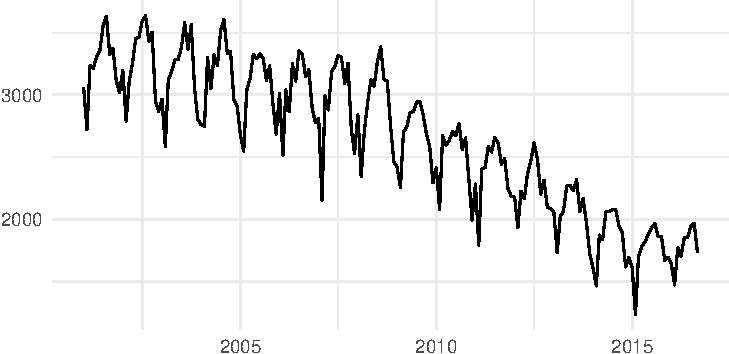
\includegraphics{Assessment_1v6_files/figure-latex/fig-1.pdf}
\caption{Crimes evolution}
\end{figure}

Except for the deceptive practice, all the crimes have decresead in more
or less grade.

\begin{figure}[htbp]
\centering
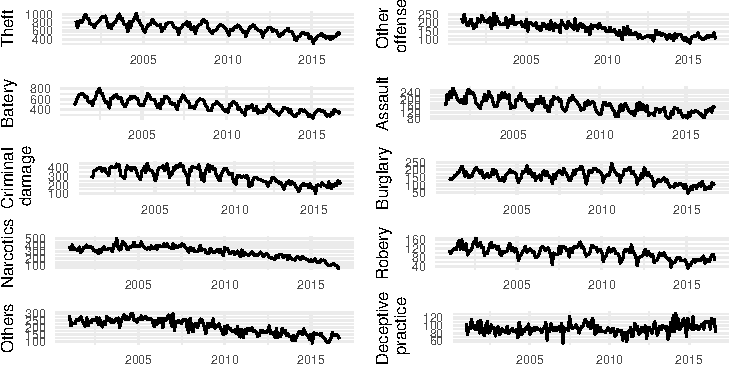
\includegraphics{Assessment_1v6_files/figure-latex/fig2-1.pdf}
\caption{Evolution per type of crime}
\end{figure}

\paragraph{Crime per Hour}\label{crime-per-hour}

The crimes are concentrated in hours

\begin{figure}[htbp]
\centering
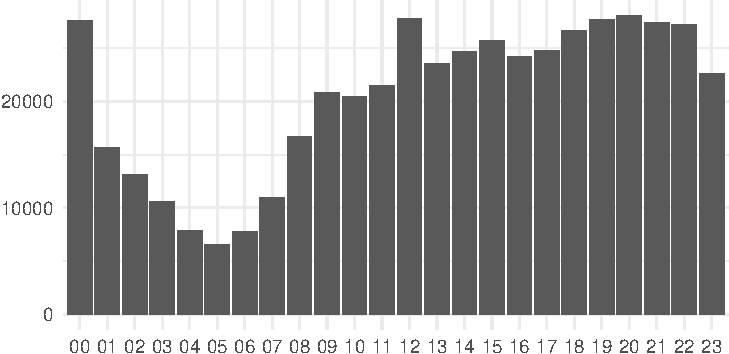
\includegraphics{Assessment_1v6_files/figure-latex/fig3-1.pdf}
\caption{Crimes per hour}
\end{figure}

\paragraph{Crime per weekday}\label{crime-per-weekday}

Friday concentrated most of the crimes, percentage?

\begin{figure}[htbp]
\centering
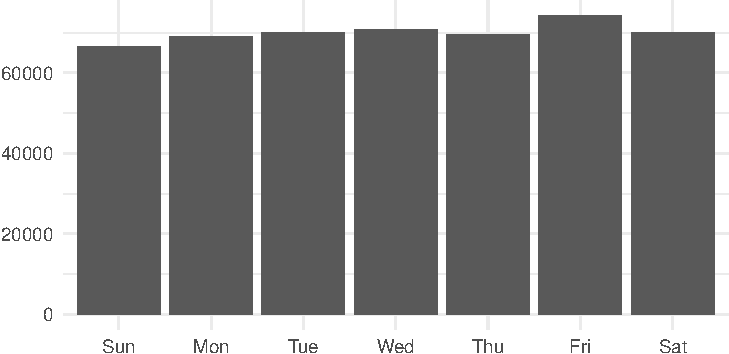
\includegraphics{Assessment_1v6_files/figure-latex/fig4-1.pdf}
\caption{Crimes per weekday}
\end{figure}

\paragraph{Crime per month}\label{crime-per-month}

Summer is in difference the period with more crimes recorded.

\begin{figure}[htbp]
\centering
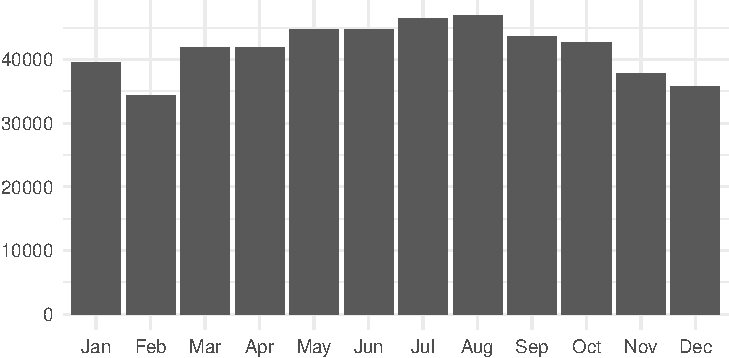
\includegraphics{Assessment_1v6_files/figure-latex/fig5-1.pdf}
\caption{Crimes per month}
\end{figure}

\paragraph{Type of crimes}\label{type-of-crimes}

Per type of crime Theft is in difference the biggest number. Change the
scientifyc number.

Change scientific numbers!

\begin{figure}[htbp]
\centering
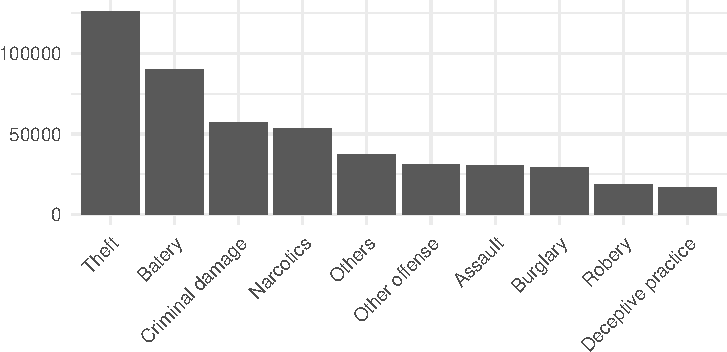
\includegraphics{Assessment_1v6_files/figure-latex/fig6-1.pdf}
\caption{Crimes per type}
\end{figure}

\paragraph{Location of crimes}\label{location-of-crimes}

These crimes are concentrated in Streets, give percentage.

\begin{figure}[htbp]
\centering
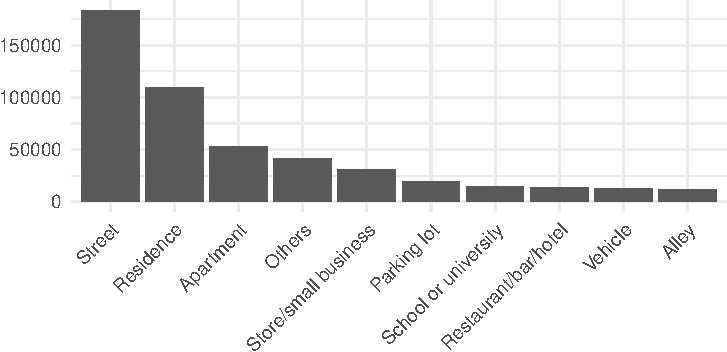
\includegraphics{Assessment_1v6_files/figure-latex/fig7-1.pdf}
\caption{Crimes per location}
\end{figure}

\paragraph{Crimes per districts}\label{crimes-per-districts}

Per districts the most dangerous are 8.

\subsubsection{Multivariable analysis}\label{multivariable-analysis}

The multiple analysis focuses on type of crime crossed with hour,
location and district.

\paragraph{Type of crime vs hour}\label{type-of-crime-vs-hour}

The most dangerous hours per Thefth are 00 and 12.

\begin{figure}[htbp]
\centering
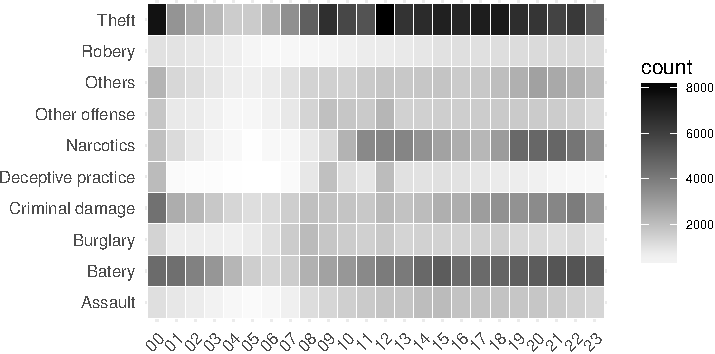
\includegraphics{Assessment_1v6_files/figure-latex/fig9-1.pdf}
\caption{Type of crime vs hour}
\end{figure}

\paragraph{Type of crime vs location}\label{type-of-crime-vs-location}

Street is particularly important for Theft.

\begin{figure}[htbp]
\centering
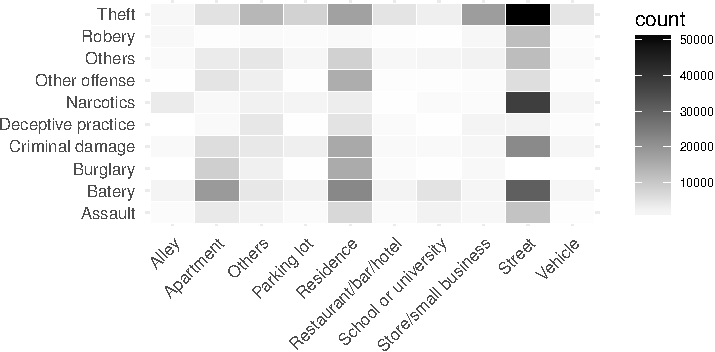
\includegraphics{Assessment_1v6_files/figure-latex/fig11-1.pdf}
\caption{Type of crime vs location}
\end{figure}

\paragraph{Type of crime vs district}\label{type-of-crime-vs-district}

Narcotics in district 11 is crealy a problem.

\begin{figure}[htbp]
\centering
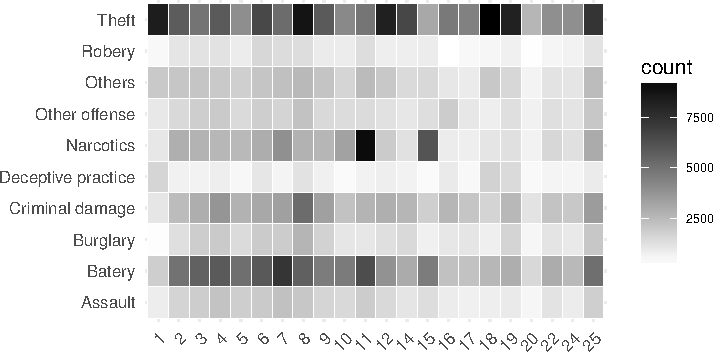
\includegraphics{Assessment_1v6_files/figure-latex/fig10-1.pdf}
\caption{Type of crime vs district}
\end{figure}

\section{Conclusions}\label{conclusions}


\end{document}
